\documentclass{article}
\usepackage{amssymb}
\usepackage{amsthm}
\def\code#1{\texttt{#1}}
% Language setting
% Replace `english' with e.g. `spanish' to change the document language
\usepackage[english]{babel}

% Set page size and margins
% Replace `letterpaper' with`a4paper' for UK/EU standard size
\usepackage[letterpaper,top=2cm,bottom=2cm,left=3cm,right=3cm,marginparwidth=1.75cm]{geometry}

% Useful packages
\usepackage{amsmath}
\usepackage{graphicx}
\usepackage[colorlinks=true, allcolors=blue]{hyperref}

\title{Option Pricing}
\author{Sean Conlon}

\begin{document}
\maketitle

%%
\section{Introduction}

So, what is Stochastic Calculus and why do we care? Stochastic calculus is the area of mathematics that deals with processes containing a stochastic component and thus allows the modeling of random systems. Many stochastic processes are based on functions which are continuous, but nowhere differentiable. This rules out differential equations that require the use of derivative terms, since they are unable to be defined on non-smooth functions. Instead, a theory of integration is required where integral equations do not need the direct definition of derivative terms. 

\section{Random Walks}
Perhaps the most simple stochastic process is the simple random walk defined as 
$$Y_t = \sum_{i=1}^{t}\xi_i$$
With $\xi_i$ being independent and identically distributed random variables with $$\mathbb{P}(\xi_i = \pm 1) = 1/2$$
Some natural questions arise from this definition, such as the expectation and variance of the walk
\begin{align*}
    \mathbb{E}[Y_t] &=  \mathbb{E}\left[\sum_{i=1}^{t}\xi_i\right] \\
    &= \sum_{i=1}^{t}\mathbb{E}[\xi_i] = 0
\end{align*}
The variance can also be determined by taking the second moment of the random variable that defines the walk
\begin{align*}
    \mathbb{E}[Y_t^2] &= \mathbb{E}[Y_t Y_t]\\
    &= \mathbb{E}\left[\sum_{i=1}^{t}\sum_{j=1}^{t}\xi_i \xi_j \right] \\
    &= \sum_{i=1}^{t}\sum_{j=1}^{t}\mathbb{E}[\xi_i \xi_j ]
\end{align*}
so long as $i\neq j$, by the independence assumption we have $\xi_i \perp \xi_j$. We now split the sum into the case that $i=j$ and $i\neq j$. 
\begin{align*}
    \sum_{i=1}^{t}\sum_{j=1}^{t}\mathbb{E}[\xi_i \xi_j ] &= \sum_{i=j}^{t}\mathbb{E}[\xi_i^2] + \sum_{i\neq j}^{t}\mathbb{E}[\xi_i \xi_j] \\
    &= \sum_{i=j}^{t} 1 + \sum_{i\neq j}^{t}\mathbb{E}[\xi_i]\mathbb{E}[ \xi_j] \\
    &= t
\end{align*}
Thus the variance of $Y_t$ is $t$. The standard deviation from the expectation at time $t$ is given by $\sigma = \sqrt{Var(Y_t)} = \sqrt{t}$. By plotting a realisation on the simple random walk against its upper/lower standard deviation, we can see this

\begin{center}
    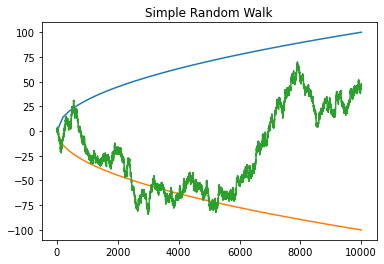
\includegraphics[scale=0.5]{images/SRR.png}
\end{center}
Making intelligent observations such as these is core to the application and study of stochastic processes, and is the purpose of applying stochastic calculus to financial asset pricing.

\subsection{Brownian Motion}
Having defined a random walk in the discrete time, we now wish to generalise to the continuous time case. The resulting walk is referred to as \textit{Brownian Motion} and plays a critical role in many continuous time models in various disciplines, particularly finance. \\
The goal is to now construct Brownian Motion, in order to do this we note that discrete random walks can be parameterised by the size of their time step $\Delta t$ and the size of the walk step $\Delta x$. From what has so far been defined, $\Delta t = 1$ along the natural number line and step size $\Delta x=1$ \\
\\
To obtain a continuous time walk $B_t$, we must have $\Delta t\longrightarrow0$. To do this let $N$ be very large and define $\Delta t = \frac{1}{N}$. Of course, we could simply let $\Delta x = \frac{1}{N}$ also, though this would be a very \textit{small} random walk, as the step size would be so small, there would be little deviation from the expectation. To preserve the level of deviation in the simple random walk desire that at each time step $t$ we have $B_t \sim \sqrt{t}N(0, 1)$ which implies
$$B_{k\Delta t} \approx \Delta x Y_k$$
Let $k=N$ and note that $B_t \sim \sqrt{t}N(0, 1)$ also implies that $B_1 \sim N(0,1) \implies \mathbb{E}[B_1] = 1$. Thus
\begin{align*}
    1 = \mathbb{E}[\Delta x Y_N^2] &= \Delta x^2 \mathbb{E}[Y_N^2] \\
    &= \Delta x^2 N
\end{align*}
$$\therefore \Delta x = \frac{1}{\sqrt{N}}$$
To verify that the Brownian Motion we have constructed matches the desired distribution $B_t \sim \sqrt{t}N(0,1)$ we express this in terms of the discrete random walk and note that there exists a $k$ such that we we have $t = \frac{k}{N}$ for all $t$
\begin{align*}
    B_t = B_{k/N} &\approx \Delta x Y_k\\
    &= \frac{1}{\sqrt{N}} Y_{k} \\
    &= \frac{\sqrt{k}}{\sqrt{N}} \frac{Y_k}{\sqrt{k}} \\
    &= \frac{Y_k\sqrt{t}}{\sqrt{k}}
\end{align*}
Recall that $Y_k$ is the sum of $k$ random variables $\xi_i$ with mean 0 and variance 1. Taking $k\longrightarrow N$ for a very large $N$ and applying the central limit theorem $\frac{Y_k}{\sqrt{k}}$ approaches a standard normal distribution. The additional coefficient $\sqrt{t}$ results in $B_t \sim \sqrt{t}N(0,1)$ as desired. \\
\\
\\
\textbf{Definition 2.1: Brownian Motion}\\
Brownian Motion is a stochastic process indexed by time with the following properties \begin{enumerate}
    \item $B_t \sim \sqrt{t}N(0,1)$ for all $t>0$
    \item if $u<t<s$ then $B_t - B_u \perp B_s - B_t$ That is, non-overlapping increments of Brownian Motion are independent from one another.
    \item $B_t$ is continuous everywhere
\end{enumerate}
We typically assume $B_0 = 0$ which is referred to as \textit{standard Brownian Motion}. \\
\\
This definition leads to our first observation about Brownian Motion and indeed stochastic calculus. This results in the following theorem on its derivative. We also provide a theorem on the \textit{quadratic variation} of $B_t$. This will provide a useful result when studying Itô's calculus, which relies on the identity. \\
\\
\textbf{Theorem 2.1: Non Differentiability of $B_t$}\\
\textit{For any t, all paths of Brownian Motion are non-differentiable with probability $1$}. 
\begin{proof}
Let $B(t)$\footnote{We use the notation $B(t)$ and $B_t$ interchangeably} be a Brownian motion and consider the definition of its derivative $B(t+\Delta) -B(t) / \Delta$. Recall that property 1 of the definition of Brownian Motion that $B(t+\Delta) -B(t) \sim N(0, \Delta) = \sqrt{\Delta}N(0,1)$ thus
\begin{align*}
    \frac{B(t+\Delta) -B(t)}{\Delta} &\stackrel{\text{d}}{=} \frac{\sqrt{\Delta} Z}{\Delta} \\
    &\stackrel{\text{d}}{=} \frac{Z}{\sqrt{\Delta}}
\end{align*}
Where $Z$ is a standard normal random variable. This ratio converges to $\infty$ in distribution, as 
$$\lim_{\Delta\longrightarrow0}\mathbb{P}\left( \left| \frac{Z}{\sqrt{\Delta}}\right| >K \right)\longrightarrow1$$
For any choice of $K$, thus precluding the existence of any derivative to $B(t)$. \\
\end{proof}

\subsection{Martingales \& Brownian Motion Martingales}
Martingales are a critical field of advanced probability theory. As we will discuss in the section on Financial Modelling, martingales guarantee a no-arbitrage result in pricing solution. Firstly, we will define what a martingale is, and the martingales of Brownian Motion. \\
\\
\textbf{Definition 2.2: Martingale} \\
A stochastic process $\{X(t), t\geq0\}$ is a martingale if for any $t\geq0$ it is integrable $\mathbb{E}[|X(t)|]<\infty$ and for any $t>s$
$$\mathbb{E}[X(t) | \mathcal{F}_s] = X(s)$$
\\
\\
The second property states that given all information about the process up to the most recent time $\mathcal{F}_s$, the best estimate of the process at future time $t$ in (expectation sense), is given by the most up to date information $X(s)$. \\
\\
The key technique if ever asked to prove that a given function of Brownian Motion $g(B(t))$ is a martingale is to show that the conditional expectation is equal to the unconditional one: 
$$\mathbb{E}[g(B(t+s)-B(t))|\mathcal{F}_t] = \mathbb{E}[g(B(t+s)-B(t))] $$
\\
\\
\textbf{Theorem 2.2: Martingales of Brownian Motion}\\
\textit{Let $B(t)$ be Brownian Motion. Then \begin{enumerate}
    \item $B(t)$ is a martingale
    \item $B(t)^2 -t$ is a martingale\footnote{This martingale actually leads to the following characterisation of Brownian Motion, a continuous process $X(t)$ is Brownian Motion if and only if $X(t)^2-t$ is a martingale. It is often difficult to show that a continuous process $X(t)$ satisfies the definition of Brownian Motion directly. In such cases, inspecting if $X(t)$ satisfies this characterisation is a common approach.}
    \item For any $u$, $e^{uB(t)-\frac{u^2}{2}t}$ is a martingale
\end{enumerate}}
\begin{proof}
By definition $B(t)\sim N(0,t)$ so by definition, standard Brownian Motion has bounded expectation. The absolute value of the process therefore also has bounded expectation $\mathbb{E}[|B(t)|]<\infty$. For a more rigorous argument, the process $|B(t)|$ follows a \textit{folded normal distribution} with variance $t$, which has expectation $\sqrt{2t/\pi}$. \\
\\
To verify the martingale property let $s>0$ and it follows
\begin{align*}
    \mathbb{E}[B(t+s)|\mathcal{F}_t] &= \mathbb{E}[B(t)+(B(t+s)-B(t))|\mathcal{F}_t] \\
    &= \mathbb{E}[B(t)|\mathcal{F}_t] + \mathbb{E}[B(t+s)-B(t)|\mathcal{F}_t] \\
    &= B(t)
\end{align*}
The second term, $\mathbb{E}[B(t+s)-B(t)|\mathcal{F}_t]=0$, as $B(t+s)-B(t)$ is an independent Brownian Motion on the interval $[t, t+s]$ which is independent of $\mathcal{F}_t$. By definition, the expectation of Brownian Motion on any interval equals to 0.\\
\\
We now show that $B(t)-t$ is a martingale. The boundedness requirement follows a similar argument from the first martingale. To show the martingale property \begin{align*}
    \mathbb{E}[B(t+s)^2 | \mathcal{F}_t] &= 
\end{align*} 
\end{proof}
\subsubsection*{Theorem 2.3: Covariance of Brownian Motion}\\
\textit{Let $B_t$ be Brownian Motion, then }$\text{cov}(B_t, B_s) = \min (t,s)$
\begin{proof}
Recall that for a random variables $X(s), X(t)$ we have cov$(X(t), X(s)) = \mathbb{E}[X(t)X(s)]-\mathbb{E}[X(t)]\mathbb{E}[X(s)]$. Assume $s<t$ and note that 
$B_t B_s = B_t^2+B_t(B_s - B_t)$ It now follows that \begin{align*}
    \text{cov}(B_t, B_s) &= \mathbb{E}[B_t B_s] - \mathbb{E}[B_t]\mathbb{E}[B_s] \\
    &= \mathbb{E}[B_s^2+B_s(B_t - B_s)] \\
    &= \mathbb{E}[B_s^2] + \mathbb{E}[B_s(B_t - B_s)] \\
    &= s + \mathbb{E}[B_s]\mathbb{E}[B_t - B_s] \\
    &= s
\end{align*}
We use the independent-increment property with the assumption that $s<t$. If we repeat with $t<s$, we achieve an expectation of $t$. Thus, Cov$(B_t, B_s) = \min(B_t, B_s)$ \\
\end{proof}
This theorem provides another characterisation of Brownian Motion, where a continuous process $X(t)$ is Brownian Motion if and only if it is a Gaussian process and has covariance with itself at times $s$ and $t$ is $\min(s,t)$


\newpage
\section{Itô Calculus}
Having constructed the Brownian Motion and defining the notion of a martingale, we are now ready to explore stochastic calculus. We keep in mind, the purpose of studying this type of calculus is to perform analysis of functions $f$, that contain random components, such as $B_t$. This will arise in financial applications, as we model asset pricing as $f(B_t)$. In fact, we often which to estimate infinitesimal movements in $f$, based on infinitesimal movement in $t$. What we have just described is the derivative of $f$ which is given by the chain rule of calculus
$$\frac{df}{dt} = \frac{df}{dB_t} \frac{dB_t}{dt}$$
however, we know from \textbf{Theorem 2.1} that the derivative $dB_t/dt$ does not exist. Another approach is to approximate it with 
\begin{align*}
    \frac{df}{dB_t} = f'(B_t) \\
    \implies df = f'(B_t)dB_t
\end{align*}
Which is no usable, as there is not $dB_t/dt$ term. Consider a Taylor series expansion of $f$
$$df = f(x+dx)-f(x) = dx f'(x) + \frac{(dx)^2}{2}f''(x) + \dots$$
let $x=B_t$ and we have 
$$= dB_t f'(B_t) + \frac{(dB_t)^2}{2}f''(B_t) + \dots$$
By the quadratic variation of Brownian Motion, we have $dB_t^2 = dt$ and higher order terms vanish. Thus the Taylor series truncates to
$$df = f'(B_t)dB_t + \frac{1}{2}f''(B_t)dt$$
\\
\textbf{Theorem 3.1: Itô's Lemma}\\
\textit{Let f be a smooth function of Brownian Motion, $f(B_t)$. Then it's differential is defined as}
$$df = f'(B_t)dB_t + \frac{1}{2}f''(B_t)dt$$
\textit{If f is a smooth function of two variables $f(t, x)$ with $B_t$ taking the value of the second variable, then }
\begin{align*}
    df(t, B_t) &= \frac{\partial f}{\partial t} dt + \frac{\partial f}{\partial x} dB_t + \frac{1}{2}\frac{\partial^2 f}{\partial x^2}dB_t^2 \\
    &= \left(\frac{\partial f}{\partial t} + \frac{1}{2}\frac{\partial^2 f}{\partial x^2}  \right)dt + \frac{\partial f}{\partial x} dB_t
\end{align*}
\textit{Or even more gernally, if $X(t)$ is a random process of Brownian Motion and $f$ is a twice differentiable function then
$$df(X(t)) = f'(X(t))dX(t) + f''(X(t))dX(t)$$}
\\
As we saw in it's derivation, Itô's lemma serves as a stochastic equivalent to the chain rule of ordinary calculus, which in turn, enables for differential analysis of smooth functions of random process'. From this rule, the basis of a stochastic calculus is formed. The third and most general statement of the lemma will also be useful in modelling stochastic processes as differential equations\\
\\
\\
\textbf{Definition 3.1: Stochastic Integration} \\
\textit{if $B_t$ is Brownian motion on a positive real interval $[0, T]$ and $f$ is a twice differentiable function, then for any $t\leq T$}
$$f(B(t)) = f(0) + \int_0^t f'(B_s)dB_s + \int_0^t \frac{1}{2}f''(B_s)ds$$
\textbf{Theorem 3.2: Differentials in Itô Calculus} \\
\textit{Under Itô calculus, the follow when performing stochastic integration of Itô's lemma \begin{enumerate}
    \item $dt^2 = 0$
    \item $dtdB_t = 0$
    \item $dB_t^2 = dt$
\end{enumerate}}
A rigorous proof of each of these requires measure theory, and therefore are often presented as a fact, rather than a theorem. However, there is a bit of intuition behind these rules that we will outline below. Recall that Itô's lemma is derived from the Taylor series expansion of $df := f(x+dx)-f(x)$ with $x = B_t$
$$df = f'(B(t))dB_t + \frac{1}{2}f''(B_t)(dB_t)^2 + \dots$$
Hence, the interest in the term $dB_t^2$, and in the multivariate case of a function $f(t, B_t)$, the differential $dtdB_t$ will appear. \\
\\
Calculus, both ordinary and stochastic, is the analysis of functions during infinitesimally small time steps, $dt$. In a similar manner, we can think of $dB_t$ as the changes that Brownian Motion makes on this infinitesimally small interval. If we separate the interval into $N$ time steps, then $dt\sim \frac{1}{N}$ and thus $dt^2 \sim \frac{1}{N^2}$. Taking $N\longrightarrow \infty$, the $dt^2$ term vanishes much faster than $dt$ and thus the first rule of Itô calculus $dt^2=0$. \\
\\
Referring back to \textbf{chapter 2}, in the construction of Brownian Motion from the simple random walk, we scale the step size $dB_t$ to be on the order of $dB_t\sim \sqrt{1/N} = \sqrt{dt}$. In other texts, it is common to see this denoted as $dB_t = O(\sqrt{dt})$. Hence, we have the identity $dB_t^2 = (\sqrt{dt})^2 = dt$.\\
\\
In similar fashion to the first argument, if $dB_t \sim \sqrt{dt}$ then $dtdB_t\sim dt^{3/2}$, which will also vanish much faster than $dt$ with $N\longrightarrow\infty$. Again, each of these serve only as an intuition and not a rigorous proof, though hopefully provides some comfort in the results of Itô calculus.\\ 
\\
\\
Another goal of stochastic calculus is to define the stochastic integral $\int_{0}^{t}X(t)dB_t$. The integral should have the all the usual properties of integration from ordinary calculus, such that if $X(t)=c$ then $\int_{0}^{t}cdB_t = c\int_{0}^{t}dB_t = c(B_t - B_0)$. Similarly, the integral over any subintervals of $[0, t]$ such that  $\int_{0}^{t}X(t)dB_t = \int_{0}^{a}X(t)dB_t + \int_{a}^{t}X(t)dB_t $. It is important to define and study such integrals as they arise from applying the stochastic integration variant of Itô's lemma. Typically, the process $X(t)$ will be a smooth function $f$ of the form $f(B_t)$.\\
\\
\textbf{Theorem 3.3: Itô Integral}\\
\textit{Let $X(t)$ be a regular stochastic process such that $\int_{0}^{t}X(t)dt<\infty$. Then the Itô integral is defined and has the following properties. \begin{enumerate}
    \item if X(t) and Y(t) form defined Itô integrals and a and b are some constants then $$\int_{0}^{t}aX(t) + bY(t)dB_t = a\int_{0}^{t}X(t)dB_t + b\int_{0}^{t}Y(t)dB_t$$
    \item The integral has zero mean
    $$\mathbb{E}\left(\int_{0}^{t}X(t)dB_t \right)=0$$
    \item Isometry
    $$\mathbb{E}\left(\int_{0}^{t}X(t)dB_t \right)^2 = \int_{0}^{t}\mathbb{E}[X(t)^2]dt$$
\end{enumerate}}
\newpage
\textbf{Theorem 3.3: Martingale Property of the Itô Integral}\\
\textit{Let X(t) be a process such that the Itô integral $\int_{0}^{t}X(t)dB_t$ is defined. Then, th Itô integral is a martingale.} 
\begin{proof}
As $X(t)$ forms an Itô integral we must have $\int_{0}^{t}X(t)^2dt<\infty$, and the integrability condition is satisfied. Suppose that $s<t$
\begin{align*}
Y(t) :&= \mathbb{E}\left(\int_{0}^{t}X(u)dB_u | \mathcal{F}_s\right) \\
   &= \int_{0}^{s}X(u)dB_u  +  \mathbb{E}\left(\int_{s}^{t}X(u)dB_u | 
\mathcal{F}_s\right) \\
&= \int_{0}^{s}X(u)dB_u = Y(s)
\end{align*}
where the expectation is cancelled by the zero-mean property of the Itô Integral. \\
\end{proof}
The focus of this document is to present the fundamental mathematics of Stochastic Calculus, under the motivation of application to derivative pricing. Naturally, one may question why we care if such integrals are martingales? The answer, as we will see, is that integral components arise often in the pricing equation of a financial derivative or security. With further motivation and explanation provided later, we desire that the pricing of a financial derivative be a martingale, therefore it is reassuring to confirm that Itô integrals are indeed martingales. 

\newpage
\subsection{Stochastic Differential Equations}
In ordinary calculus, differential equations are used to describe the evolution of a system. Their stochastic counterpart arise when a random noise is introduced to ordinary differential equations (ODE's). Let $B_t$ be Brownian Motion, an equation of the form 
$$dX(t) = \mu(X(t), t)dt + \sigma(X(t), t)dB_t$$
is an SDE, where functions $\mu(X(t), t)$ and $\sigma(X(t), t)$, known as the drift and diffusion coefficient respectively are given, and $X(t)$ is an unknown process that we must solve for. Note that if $\sigma=0$, the differential equation truncates to a classical ODE. \\
\\
Stochastic systems, such as asset prices, bond/equity volume flows, infection transmission are typically modelled using equations of the above form. We present some common SDEs and provide their solution, which is obtained using Itô's lemma. 

\subsubsection{Geometric Brownian Motion}
A common model for the spot price $S(t)$ of a financial asset at time $t$, geometric Brownian Motion is the solution to the following SDE
$$dS(t) = \mu S(t)dt + \sigma S(t)dB_t \quad \quad S(0) = S_0$$
Where the constant $\mu$ represents the long term \textit{percentage drift} of the asset price, typically a positive real number in the range of $[3, 12]$, and $\sigma$ a constant representing \textit{percentage volatility}.  With practice and experimentation, one can reason about the form of the SDE and derive the correct choice of smooth function $f$ to apply in Itô's lemma to solve the equation. In the case of geometric brownian motion, we take $f(S(t)) = \ln S(t)$ and by Itô's lemma
\begin{align*}
    d(\ln S(t)) &= \frac{1}{S(t)}dS(t) - \frac{1}{2S(t)^2}dS(t)^2 \\
    &= \frac{1}{S(t)}\mu S(t)dt + \sigma S(t)dB_t - \frac{1}{2S(t)^2}(\mu S(t)dt + \sigma S(t)dB_t)^2 \\
    &= \mu dt + \sigma dB(t) - \frac{1}{2S(t)^2}(\mu^2S(t)^2dt^2 + 2\mu\sigma S(t)^2dtdB_t + \sigma^2 S(t)^2 dB_t^2)\\
    &= \mu dt + \sigma dB_t - \frac{\sigma^2}{2} dt \\
    &= \left(\mu - \frac{\sigma^2}{2}\right)dt + \sigma dB_t
\end{align*}
Let $Y(t) = \ln S(t)$ and applying stochastic integration gives $Y(t) = Y(0) + (\mu - \sigma^2)t + \sigma B_t$ substituting back $\ln S(t)$ yields 
\begin{align*}
    & \ln S(t) = Y(0) + (\mu - \sigma^2/2)t + \sigma B_t \\
    & S(t) = e^{Y(0)}e^{(\mu - \sigma^2/2)t + \sigma B_t}
\end{align*}
Solving for the boundary condition $S(0)=S_0$ and we obtain the solution
$$S(t) = S_0 e^{(\mu - \frac{\sigma^2}{2})t + \sigma B_t}$$

\subsubsection{Ornstein-Uhlenbeck Process}
Another SDE that arises often in financial applications is the so-called \textit{Ornstein-Uhlenbeck process} which takes the form
$$dX(t) = -\alpha X(t)dt + \sigma dB_t$$
with $\alpha$ and $\sigma$ non negative constants. The process is used extensively to model mean-reverting assets such as FX rates, interest rates and commodity prices. To derive its solution, we note that in the non-stochastic variation with $\sigma=0$ we have
$$dX(t) = -\alpha X(t)$$
Which has the ODE solution $X(0)e^{\alpha t}$. In otrder to solve the SDE, we conisder the process $Y(t) := X(t)e^{\alpha t}$ using the differential of the product rule
$$dY(t) = e^{\alpha t}dX(t) + \alpha e^{\alpha t}X(t)dt$$
Substituting $dX(t)$ we have $dY(t) = \sigma e^{\alpha t}dB_t$. By applying stochastic Integration we arrive at
$Y(t) = Y(0) + \int_{0}^{t}\sigma e^{\alpha t}dB_t$. And thus the solution to $X(t)$ is given by


\newpage
\section{Risk-Neutral Measures}
It as it this point our attention begins to shift towards application in derivative pricing. In probability and measure theory, the function $\mathbb{P}$ that maps the likelihood outcome of a random variable $X=x$ to the $[0,1]$ subsection of the real line is known as the \textit{probability measure}. In machine learning, applied statistics and indeed quantitative finance, we are often estimating the likelihood of an outcome,  that is to approximate $\mathbb{P}(X=x)$ given some data. Within quantitative finance communities, this measure $\mathbb{P}$ is often
referred to as the \textit{observed} or \textit{real world} measure that we see reflected in securities prices. As we see below, there is a deep connection between the existence of these risk-probability measures, and asset pricing.\\
\\
\textbf{Theorem 4.1: Girsanov Theorem}\\
\textit{Let X, Y be continuous martingales under a probability measure $\mathbb{P}$. Define M to be solution to the SDE
$$M_{t}=1+\int_{0}^{t} M_{s} d X_{s}=\exp \left(X_{t}-[X]_{t} / 2\right)$$
Provided M is sufficiently integrable, one can define a new measure $\mathbb{Q}$ by $\mathbb{Q}(A) = \mathbb{E}_{\mathbb{P}}[1_{A}M_T]$ and under the new new measure $$Y_t - \int_{0}^{t}X_t dY_t$$ is a continuous, local martingale. } \\
\\
It is not immediately obvious how Girsanov theorem can be of practical use in application to finance. In practice, this theorem is applied quite extensively, typically to show if $dX_t = H_s dB_t$ and $Y_t = B_t$ for a Brownian Motion under some real-world measure $\mathbb{P}$, then there exists a measure $\mathbb{Q}$ such that $B_t - \int_{0}^{t}H_sds$ is a martingale. Another theorem that will be applied to obtain derivative pricing is the so-called martingale representation theorem. \\
\\
\textbf{Theorem 4.2: Martingale Representation Theorem}\\
\textit{Let $B_t$ be a standard Brownian Motion. Then every $\mathcal{F}_t$ local martingale $X$ can be written as 
$$X(t) = X(0) + \int_{0}^{t}H(s)dB_s$$}\\

\subsection{Fundamental Theorem of Asset Pricing}
The fundamental theorem of asset pricing provides necessary and sufficient conditions for a market to be \textit{arbitrage-free} and \textit{complete}. We have so far defined what it means for a market to be arbitrage-free; there is an absence of arbitrage opportunities. A market is said to be \textit{complete}, if there exists a replicating portfolio for any financial asset, which is a desirable property.
\\
\\
\textbf{Theorem 5.2: Fundamental Theorem of Asset Pricing}
\textit{\begin{enumerate}
    \item A discrete market on a discrete probability space is arbitrage-free if, and only if, there exists at least one risk-neutral probability measure that is equivelant to the original measure $\mathbb{P}$
    \item An arbitrage-free market consisting of a universe of securities $S$ and risk-free instruments $B$ is complete if, and only if, there exists a unique risk-neutral measure with numeraire $B$
\end{enumerate}}
The first item of the theorem is important for when pricing financial derivatives, as it provides a means of ensuring that prices are arbitrage-free and we (the market maker) can avoid exploitative behaviour from market participants. 

\newpage
\section{Introduction to Options Pricing}
Having developed the theories of a stochastic calculus, we know look to apply them to the financial domain, particularly in the pricing of financial derivatives. When pricing a financial asset, we are doing so from the perspective of the market maker; that is, we wish to continuously determine price quotes for market participants, both buyers and sellers. The following \href{https://www.youtube.com/watch?v=j1oV2BTSi1s&t=0s}{video lecture} from \textit{Oxford Mathematics} provides a brilliant outline of the priorities when pricing a derivative. In the lecture, they explain the key concerns of financial modelling are (in order): 
\begin{enumerate}
    \item Avoid being exploited. 
    \item Control, manage and understanding risk. 
    \item Make a profit (usually by managing risk). 
\end{enumerate}
We will also need some economic assumptions when building financial models. The basic assumptions that underlay most models are \begin{itemize}
    \item There is a riskless investment (a bank account or Treasury Bond) which grows at a constant, continuously compounded rate $r$.
    If $M_t$ is invested at time $t$, then it grows to $M_T = M_t e^{r(T-t)}$ at time $T>t$. 
    \item Trading is \textit{friction-less}, meaning that there is no trading costs, and impact on volume when buying at time $t$.
    \item Assets are infinitely divisible. This is a technical condition to enable pricing functions on $\mathbb{R}$. In practice, it is common to see derivative products structured this way. 
\end{itemize}
The key concepts to financial mathematics which will allow us to build arguments is arbitrage, which formalises the concept of an exploitable investment opportunity. \\
\\
\textbf{Definition 5.1: Arbitrage} \\
An \textit{arbitrage} is an investment $X_t$ which costs nothing (or less) at time $t$, $X_t\leq0$ though later at time $T>t$ has: \begin{enumerate}
    \item zero probability of negative value, $\mathbb{P}(X_T <0)=0$
    \item strictly non-zero probabilty of having strictly positive value, $\mathbb{P}(X_T >0)>0$
\end{enumerate}
Note these two conditions imply that $X_t$ generates a riskless, positive profit as $\mathbb{P}(X_T =0)=0$. When modelling, we assume that \textit{no arbitrage opportunities exist}. In practice they do, though they are quickly exploited and supply and demand causes prices to realign in order to eliminate them. \\
\\
The no-arbitrage principal is also seen as the \textit{law of one price}. If there exists two ways of constructing a payoff within the market, and one of them is cheaper than the other, then we can construct a portfolio which
\begin{itemize}
    \item Buys a cheaper version of the claim, (short) sells the more expensive. 
    \item At expiry, has no risk but has made an initial profit.
\end{itemize}
With the notion of arbitrage defined, we can now turn to pricing some financial derivatives. For initial simplicity, let us consider pricing a derivative on an equity (shares of companies) that cost nothing to hold. \\
\\
\textbf{Definition 5.2: Call \& Put Option}\\
A call option is a contract with expiry date $T>t$ and a strike $K>0$ which: \begin{itemize}
    \item the holder (long position) has the \textit{right but not the obligation} to buy the underlying at time $T$ for price $K$ 
    \item the writer (short position) has the \textit{obligation} to deliver the underlying to the holder at time $T$ for price $K$ in the event that the holder exercises. 
\end{itemize}
The value of the long position at time of expiry is 
$\max(S_T-K, 0) = (S_T-K)^+$
A put option is defined similarly, though with the holder (long position) has the \textit{right but not the obligation} to sell the underlying at expiry. The value of the long position at time $T$ is therefore
$\max(K-S_T, 0) = (K-S_T)^+$ \\
\\
\\
Different options have different exerices times. The most basic form of option, a \textit{European} grants the long position the right to exercise their option only at the time of expiry. The more common, though equally more difficult to price \textit{American} style grants the long position to exercise at any time $t\leq T$. Another term used when discussing options is \textit{moneyness}, defined below \\
\\
\textbf{Definition 5.3: Moneyness} \\
\textit{Moneyness} refers to the intrinsic value of an option in its current state, that is, the payoff the option provides if it were to expire immeditaly with strike price $K$ and value of the underlying, $S_t$. We describe the moneyness of an option as \begin{itemize}
    \item In the money (ITM), if the ratio $S_t/K>1$
    \item At the money (ATM), if the ratio $S_t/K=1$
    \item Out of the money (OTM), if the ratio $S_t/K<1$
\end{itemize} 
\\
\\
With the notion of options defined, as well as their exercise styles and the no-arbitrage goal of pricing, we can define our first theorem on option pricing. \\
\\
\textbf{Theorem 5.1: Put-Call Parity}\\
\textit{Consider a European Call and European Put option, written on the same underlying with spot price $S_t$ with the same maturity $T$. Suppose the risk-free discount factor from $t$ to maturity $T$ is $e^{r(T-t)}$ and there is no default risk. Then their respective prices $C_t$ and $P_t$ at time $t<T$ must satisfy
$$C_t - P_t = S_t - Ke^{-r(T-t)}$$
or there exists an arbitrage.}
\begin{proof}
Consider purchasing a single call and single put, for initial cost $C_t - P_t$. This portfolio generates no cash flows up until time $T$ at which it delivers payoff
$$C_T - P_T = (S_T - K)^+ - (K - S_T)^+ = S_T - K$$
While its value is unkown, the payoff is identical, in every state of the world to a portfolio consisting of one stock and debt of $K$ at time $T$. At time $t<T$ the latter portfolio has value
$$S_t-K e^{-r(T-t)}$$
If these two initial portfolios where to have different prices, then an arbitrage opportunity could be exploited by selling the more expensive and buying the cheaper. Thus we must have $C_t - P_t = S_t - Ke^{-r(T-t)}$ \\ 
\end{proof}


\subsection{Continuous Time Market Model}
We know look at a continuous time model for pricing a European call/put option at time $t<T$. We assuming an underlying equity with spot price $S_t$, and there exists a bond/savings account $W_t$\footnote{In some texts it is common to denote this \textit{bond account} as $B_t$, though this conflicts with previous chapters use of $B_t$ to denote \textit{Brownian Motion}.} that satisfies $dW_t = rW_tdt$. \\
\\
We assume that $S_t$ evolves according to the stochastic differential equation
$$\frac{dS_t}{S_t} = (\mu - q)dt + \sigma dB_t$$
Where $\mu$ is the long-term drift, $q$ is the continuous dividend yield and $\sigma>0$
is the volatility. Over each infinitesimal period $[t, t+dt)$ the share pays $qS_tdt$ in dividends. This is a poor, though widely deployed and used model for dividend paying shares. For simplicity, we assume that dividends are reinvested as they are compounded which is the rate $e^{qt}$, thus the total value of the equity position at $t$ is given by $p_t = e^{qt}S_t$. Applying Ito's lemma
We assume that $S_t$ evolves according to the stochastic differential equation
$$\frac{dp_t}{p_t} =  \mu dt + \sigma dB_t$$
Tradiing strategies are given by random processes. If at the start of the period $[t, t+dt)$ we hold $H_t$ volume of shares, then at the end of the increment, our wealth will be $H_t(S_{t+dt} - S_t)$. If we add these periods together and take $dt\longrightarrow0$ we obtain the stochastic integral 
$$\int_{0}^{t}H_u dS_u$$
For describing the gains from trading the asset. By connecting choice for $H_t$ to a solution of a PDE, we can find trading strategies $H$ that eliminate the risk of holding an option, which allows us to use the no-arbitrage assumption to determine prices. 

\subsection{Hedging, Replication \& Black-Scholes Equation}
We can obtain a price for an option using a hedging and no-arbitrage argument. Let $V_t$ denote the price of a call option on underlying security with spot price $S_t$. At expiration, we must have $V_T = (S_T - K)^+$, though at time $t<T$, we must have the value of the option being a function of time and spot price, $V_t = V(S_t, t)$. \\
\\
Assume that underlying asset follows a geometric Brownian Motion $\frac{dS_t}{S_t} = \mu dt + \sigma dB_t$ and apply Ito's lemma (for a function of two variables) to $V_t$ to obtain the following equation
$$dV = \left(\mu S_t\frac{\partial V}{\partial S_t} + \frac{\partial V}{\partial t} + \frac{1}{2}\sigma^2 S_t^2\frac{\partial^2 V}{\partial S_t^2} \right)dt + \sigma S_t \frac{\partial V}{\partial S_t}dB_t$$
Now construct a so-called \textit{delta hedged}\footnote{The portfolio is \textit{delta hedged} as it grants exposure to the option without the \textit{delta risk}, which is the risk that comes with holding a derivative associated with changes to the price of the underlying. More on such risk measures later} portfolio at time $t$ that consists of one short position in the option, and long $\partial V / \partial S_t$ untis in the underlying. The value of the portfolio, $\Pi$ is given by
$$\Pi = -V + \frac{\partial V}{\partial S_t}S_t$$
Over the time period $[t, t+\Delta t]$, the value of the portfolio changes according to
$$\Delta\Pi = -\Delta V + \frac{\partial V}{\partial S_t}\Delta S_t$$
Discretising the equation for $dS_t/S_t$ and $dV$ we have 
\begin{align*}
    & \Delta S_t = \mu S_t\Delta t + \sigma S_t \Delta B_t \\
    & \Delta V = \left(\mu S_t\mu\frac{\partial V}{\partial S_t} + \frac{\partial V}{\partial t} + \frac{1}{2}\sigma^2 S_t^2\frac{\partial^2 V}{\partial S_t^2} \right)\Delta t + \sigma S_t \frac{\partial V}{\partial S_t}\Delta B_t
\end{align*}
Substituting these expressions for $\Delta S$ and $\Delta V$ into the equation for the delta hedged portfolio and we yield 
$$\Delta \Pi = \left( -\frac{\partial V}{\partial t}-\frac{1}{2}\sigma^2 S_t^2\frac{\partial^2 V}{\partial S_t^2}\right)\Delta t$$
Notice that the $\Delta B_t$ term has vanished, thus eliminating any uncertainty rendering the portfolio riskless, effectively constructing a replicating portfolio for the risk free rate, $r$. By the \textit{law of one price} principal for no arbitrage, we must have the risk free rate over the period $[t, t+\Delta t]$ compounding to $r\Pi\Delta t = \Delta \Pi$. By substituting and rearranging we obtain
\begin{align*}
    & \Delta \Pi = r\Pi\Delta t \\
    & \left( -\frac{\partial V}{\partial t}-\frac{1}{2}\sigma^2 S_t^2\frac{\partial^2 V}{\partial S_t^2}\right)\Delta t = r\left( -V + \frac{\partial V}{\partial S_t}S_t \right) \Delta t \\
    & \frac{\partial V}{\partial t} + \frac{1}{2}\sigma^2 S_t^2\frac{\partial^2 V}{\partial S_t^2} + rS_t  \frac{\partial V}{\partial S_t} -rV = 0
\end{align*}
Therby arriving at the celebrated Black-Scholes partial differential equation. Suppose like we have assumed in section \textbf{4.1} that the underlying pays a continuous dividend yield $q$, then we can reproduce the Black-Scholes equation with a few minor adjustments. Instead, the difference in the value of the delta-hedge portfolio becomes 
$$\Delta\Pi = -\Delta V + \frac{\partial V}{\partial S_t}\Delta S_t + q S_t\frac{\partial V}{\partial S_t}dt $$
And again, by following the subsitution and rearrangement trick, we arrive at 
$$\frac{\partial V}{\partial t} + \frac{1}{2}\sigma^2 S_t^2\frac{\partial^2 V}{\partial S_t^2} + (r-q)S_t  \frac{\partial V}{\partial S_t} -rV = 0$$
With the assumptions of the Black-Scholes model, the above equation holds for any option with a price function $V$ that is twice differentiable with respect to $S_t$ and once with respect to $t$. Different pricing formulae for various options will arise from the choice of payoff function at expiry and appropriate boundary conditions.
\subsection{European Options}
For particular types of derivatives with specific payoff's and boundary condition, the black-scholes PDE has a closed form solution. One such derivative is a European call option. By Put-Call Parity, we can then derive a prive of the corresponding put option.\\ 
\\
Recall that a European call option allows the holder (the long position) the right but not the obligation to purchase the underlying $S_t$ at expiry $T$ for strike price $K$. One way to derive a solution is to notice that 
\begin{align*}
    \max(S_T-K, 0) &= (S_T-K)1_{\{S_T>K\}} \\
    &= S_T 1_{\{S_T>K\}} - K 1_{\{S_T>K\}}
\end{align*}
We now find a suitable expression for both components on the right hand side. First, we show that if $X = \exp{(a+bZ)}$ where $Z\sim N(0,1)$ and $b>0$ we can compute
\begin{align*}
    \mathbb{E}[1_{\{ \exp{(a+bZ)>K}\}} ] &=  \int  1_{\{ \exp{(a+bZ)>K}\}} \frac{1}{\sqrt{2\pi}}e^{\frac{-z^2}{2}}dz \\
    &=  \int  1_{\{ {Z>\frac{\log(K)-a}{b}}\}} \frac{1}{\sqrt{2\pi}}e^{\frac{-z^2}{2}}dz \\
    &= 1 - \Phi\left(\frac{\log(K)-a}{b}\right) \\
    &= \Phi\left(\frac{a-\log(K)}{b}\right)
\end{align*}
A similar calculation, made easier by noticing that 
$$a+bz - \frac{z^2}{2} = a+\frac{b^2}{2}-\frac{(z-b)^2}{2}$$
gives for $X = \exp{(a+bZ)}$
\begin{align*}
    \mathbb{E}[X1_{\{ \exp{(a+bZ)>K}\}} ] &= \int e^{a+bz} 1_{\{ \exp{(a+bZ)>K}\}} \frac{1}{\sqrt{2\pi}}e^{\frac{-z^2}{2}}dz \\
    &= e^{a+\frac{b^2}{2}}\int 1_{\{ z-b> \frac{\log(K)-a}{b}-b\}} \frac{1}{\sqrt{2\pi}}e^{\frac{-(z-b)^2}{2}}dz \\
    &= e^{a+\frac{b^2}{2}}\Phi\left( \frac{\log(K)-a}{b}+b\right)
\end{align*}
AS $S_T$ is assumed to follow a geometric Brownian motion, we know that for some $Z\sim N(0,1)$
\begin{align*}
    S_T &= S_t \exp\left(\left( r+\frac{\sigma^2}{2}\right)(T-t) + \sigma(B_T - B_t) \right) \\
    &= \exp\left(\log(S_t) + \left( r+\frac{\sigma^2}{2}\right)\tau + \sigma\sqrt{\tau}Z \right)
\end{align*}
Where we make the usual subsitition of $\tau:= T-t$. Using this, the discounted prices of the two components in the initial equation simplify to
\begin{align*}
    & e^{-r\tau}\mathbb{E}_{\mathbb{Q}}[ K 1_{\{S_T>K\}}|S_T = S] = e^{-r\tau} K \Phi(d_{-}) \\
    & e^{-r\tau}\mathbb{E}_{\mathbb{Q}}[ S_T 1_{\{S_T>K\}}|S_T = S] = S e^{-q\tau} \Phi(d_{+})
\end{align*}
Where $\Phi(x)$ is the CDF of a standard normal distribution evaluated at $x$ and 
$$d_{\pm} = \frac{\log(S/K) + (r-q \pm \frac{1}{2}\sigma^2)\tau}{\sqrt{\sigma^2\tau}}$$
and so, the value of a Call Option under the Black-Scholes model is
$$V^{BS} = S_t e^{-q\tau}\Phi(d_+) - Ke^{-r\tau}\Phi(d_-)$$

\subsection{Arbitrage-Free Pricing in the Black-Scholes Model}
The motivation for studying and creating mathematical models of financial derivatives is to prevent us being exploited and to understand our risk; chief among the forms of exploitation is arbitrage. Fortunetly, the Black-Scholes model satisfies the no-arbitrage condition of the fundamental theorem of asset pricing, by producing a unique risk-neutral measure. This means that the Black-Scholes model is also complete, in the sense that any payoff can be replicated. \\
\\
\textbf{Theorem 5.3: Risk Neutral Evaluation in Black-Scholes} \\
\textit{Suppose we have a Black-Scholes model. Then there exists a unique probability measure $\mathbb{Q}$ such that every traded European option claim $X_t$ has no-arbitrage time $t<T$ price 
$$X_t = e^{-r(T-t)}\mathbb{E}_{\mathbb{Q}}[X_T | \mathcal{F}_t]$$
that is, the discounted price $e^{-r(T-t)}$ is a martingale under the measure $\mathbb{Q}$.}
\begin{proof}
Under the Black-Scholes model, we assume that the price of an asset $S_t$ changes according to 
$$\frac{dS_t}{S_t} = \mu dt + \sigma dB_t$$ where $B_t$ is a Brownian Motion under the real-world probability measure $\mathbb{P}$. As we have seen before, this SDE solves to 
$$S_t = S_0 e^{(\mu - \frac{1}{2}\sigma^2)t + \sigma B_t}$$
\end{proof}

\subsection{Observations of the Black-Scholes Model}

\newpage
\section{Measures of Price Sensitivity in the Black-Scholes Model}
Recall our main goals when mathematically modelling a financial derivative are to avoid being exploited, understand our risk, and to make a profit. By the no-arbitrage condition of the Black-Scholes model, we know that pricing options according to model prevents us being exploited by arbitraguers. Let us know shift our focus to better understanding our risk when pricing, trading and holding options. \\
\\
As we have seen, the Black-Scholes model provides a closed form pricing solution to the value of a European option, using several inputs  $V^{BS}(S_t, T, r, K, \sigma)$. Over the lifetime of an option, the values of some of the inputs can change, particularly the price of the underlying $S_t$, the volatiltiy of the underlying $\sigma$ and the risk-free rate, $r$. If we hold an options contract (which we do in significant volume as a market maker), it is important to understand how the value of our options inventory changes with respect to changes in the inputs to the pricing function.

\subsection{The Greeks}
We are interested in understanding how the value of an option contract $V$ changes with respect to change in one of its input parameters, such as $S_t$. What we have described here is the partial derivative, $\frac{\partial V}{\partial S_t}$. There exists first and second order partial derivatives that are of interest to understanding the risk associated with an options trade. These partial derivatives are traditionally denoted by greek letters and are therefore referred to as, \textit{the greeks}. \\
\\
We assume the Black-Scholes model, which values a call option on underlying $S_t$ which pays continuous dividend yield $q$, with risk-free rate $r$, strike price $K$ and time-to-maturity of $\tau$. We have shown Black-Scholes value of the call option at time $t$ is 
$$V^{BS} = S_t e^{-q\tau}\Phi(d_+) - Ke^{-r\tau}\Phi(d_-)$$
Where 
$$d_{\pm} = \frac{\log(S/K) + (r-q \pm \frac{1}{2}\sigma^2)\tau}{\sqrt{\sigma^2\tau}}$$
\subsubsection{Delta}
Delta, $\Delta$, measures the rate of change in the theoretical value of the option, given a change in the price of the underlying asset $S_t$, in the case of the Black-Scholes equation, this derivative results in 
\begin{align*}
    \Delta :&= \frac{\partial V}{\partial S_t} \\
    &=  e^{-q\tau}\Phi(d_+)
\end{align*}

\subsubsection{Vega}
The Volatility $\sigma$ is the only parameter in the Black-Scholes model (and indeed, other models of option prices), that is not directly observed in the market. It is therefore important to be able to evaluate the dependence of option price on volatility. Vega, $\mathcal{V}$, measures the rate of change in the theoretical value of an option, given a change in the volatility of the option. 
\begin{align*}
    \mathcal{V} &:= \frac{\partial V}{\partial \sigma} \\
    &= S_t e^{-q\tau}\phi(d_+)\sqrt{\tau}
\end{align*}
Where $\phi(\cdot)$ denotes the standard normal distribution. 

\subsubsection{Theta}
The value of an option can be seen as: $V = $ intrinsic value + time value. The \textit{intrinsic value} is the value of the payoff if expired today. The \textit{time value}, refers to the amount of time an option has to expire in the money. An out of the money call option with 12 months to expiry is more valuable than a call option of the same strike with only 2 days to expiry. Theta, $\Theta$, describes how the value of an option changes with its time to maturity. 
\begin{align*}
    \Theta :&= - \frac{\partial V}{\partial \tau} \\
            &= -e^{-q \tau} \frac{S \phi\left(d_{1}\right) \sigma}{2 \sqrt{\tau}}-r K e^{-r \tau} \Phi\left(d_{2}\right)+q S e^{-q \tau} \Phi\left(d_{1}\right)
\end{align*}
Where the result is made negative to capture the decay in value an (OTM) option has as $\tau\longrightarrow0$.
 The mathematical result of the formula for theta is expressed in value per year. By convention, it is usual to divide the result by the number of days in a year, to arrive at the amount an option's price will drop, in relation to the underlying stock's price. 
 
\subsubsection{Rho}
The risk-free rate $r$, or indeed any rate that is used to price a derivative is itself a random variable that can change over the life of the option. The sensitivity of the option portfolio to changes in the rate is given by $\rho$. 
\begin{align*}
    \rho :&= \frac{\partial V}{\partial r} \\
    &= K\tau e^{-r\tau}\Phi(d_-)
\end{align*}
While rates are subject to change (see the rich theory on rates modelling), they typically do so in smaller movements of 0.25\code{bps}. This means that unless in extreme circumstances, the value of an option portfolio does not change much as the result of changes in rates. It is for this reason, that $\rho$ is typically the least used of the first-order greek derivatives.

\subsubsection{Gamma}
Gamma, $\Gamma$, is referred to as a \textit{second order greek}, as it described the sensitivity of Delta with respect to changes with respect to the underlying.
\begin{align*}
    \Gamma &= \frac{\partial}{\partial S_t}\Delta \\
           &= \frac{\partial^2 V}{\partial S_t^2} \\
           &= e^{-q \tau} \frac{\phi\left(d_{1}\right)}{S \sigma \sqrt{\tau}}=K e^{-r \tau} \frac{\phi\left(d_{2}\right)}{S^{2} \sigma \sqrt{\tau}}
\end{align*}

\subsection{Hedging an Option Portfolio}
As we  are pricing options from the perspective of the market maker, our responsibility is to continuously provide quotes to buy and sell particular options, making a profit on the spread between these prices. This also means that the market maker must always be prepared to buy or sell a particular option and must therefore manage a large portfolio of the securities, also referred to as the \textit{inventory}. \\
\\
Managing the risk of the inventory portfolio is therefore paramount to ensure that the market maker can meet their obligations to quote prices, and make trades. As we have described above, the greeks provide a quantitative measure of the risks/exposures in the portfolio. The goal of \textit{hedging} is to therefore buy/sell volumes in the underlying, or other options contracts to offset the portfolios greeks and ideally, keep them as close to 0 as possible. In doing so, the portfolio has no exposure to the movement in the securities, volatility, time decay ect. and allowing the market maker to generate risk-less profit on the spread.  \\
\\
Hedging is carried out using huerisitc strategies that are performed at the traders discretion. This typically involves a daily or weekly rebalance of the portfolio to bring certain greeks close to 0. Similarly, if price moves are fast and adversarial, then on-the-spot portfolio rebalances can be performed. 

\subsection{Summary Table of Greeks}
The Black-Scholes model gives a closed form solution for the Greeks of an option. Computationally, this is highly desirable, as it means that the risk of an options position can be assesed in $\mathcal{O}(1)$ time complexity. We provide a summary table of the first and second order Greeks for an option under the Black-Scholes model. 

\newpage
\section{Volatility Surfaces}
The Black-Scholes formula gives us the value of a European option as a function of the following inputs: \begin{itemize}
    \item The current price of the underlying security $S_t$
    \item The time to the maturity $\tau := T-t$
    \item The risk-free interest rate $r$
    \item The strike price of the option $K$
    \item The volatility of the underlying security $\sigma$
\end{itemize}
Suppose we wish to apply the Black-Scholes model to price an option. We can readily access the spot price of the underlying security $S_t$ and similarly, the time to maturity and strike price are also readily available from the option contract. How do we find the values of $r$ and $\sigma$ however? \\
\\
The Central bank typically sets a risk-free \textit{cash rate} that outlines their targeted money-market rate whilst conducting monetary policy. This rate is published and widely used by financial institutions, the \hyperlink{https://www.rba.gov.au/}{Reserve Bank of Australia} (RBA) publish their cash-rate targets online. This might suggest a good value for $r$, however this rate is not representative of the cost of \textit{borrowing}, we cannot borrow at rate $r$ in reality. Practically, $r$ is obtained from the forward price of $S_t$. Recall (from Forwards pricing) that the price of a forward on $S_t$ at maturity $T$ is 
$$F_t = e^{r(T-t)}S_t$$
and hence
$$\log(F_t/S_t) = r(T-t)$$
Which gives a representative interest rate for participants in the forward market, and is widely used for selecting $r$ in practice. Other alternatives include using the now defunct, \code{LIBOR} which was the opportunity cost risk-free rate for global banks when pricing a derivative. Alternatives such as the secured overnight funds rate (\code{SOFR}) are now beggining to proliferate.  \\
\\
How to choose $\sigma$ however? One idea is to take a point-estimate from historical data. At time $t$, we can split the observable interval into $N$ partitions of length $\delta$, so that an ubiased and efficient estimator of $\sigma$ is given by $$\hat{\sigma}^2 = \frac{1}{(N-1)\delta}\sum_{i=1}^{N}\left( \frac{S_{t_{i+1}} - S_{t_i}}{S_{t_i}}\right)^2$$
This is a natural approach, though has significant drawbacks. Volatility is non-constant in any market, over time $\sigma$ varies signficantly. The estimate becomes less reliable as we decrease $t$, whilst increasing it just gives an average of lifetime volatility. Furthermore, it captures only historical information, whereas prices include sentiment about the future. \\
\\
An alternative method is to just deduce $\sigma$ from the prices currently observed in the market. This gives rise to \textit{implied volatility}. \\
\\
\textbf{Definition 6.1: Implied Volatility}\\
Given the market price of an option, $V^{mkt}$, the implied volatility $\sigma_{imp}$ is the value such that 
$$V^{mkt} = V^{BS}(S_t, T, r, K, \sigma_{imp})$$
That is, the value for $\sigma$ that results in the Black-Scholes equation price equally market prices, where all other parameters are known. \\
\\
As $\sigma$ is the only non-observable paramter to the Black-Scholes equation, in some sense, market prices on European Options reflect market expectations for future volatility on the underlying asset\footnote{This is actually what is used to calculate the \code{VIX} index, a quantification of \textit{future volatility expectations}}. It is for this reason, that many markets quote option prices in terms of Implied Volatiltiy, and not actual dollar-cost of the option contract. How do we find implied volatility however? Practically speaking, a pricing function for an option (such as Black-Scholes) does not have a closed form solution for its inverse. Finding the implied volatility is therefore performed as a root-finding problem where all other parameters to the pricing function are observable
$$\sigma_{imp}:\quad V^{mkt} - V^{BS}(S_t, T, r, K, \sigma_{imp}) = 0$$

\subsection{Implied Smile and Volatility Surfaces}
If the Black-Scholes model assumptions were true, then would be one value of $\sigma_{imp}$ for call options of all strikes and maturities; as volatility is assumed constant over the life of the option. This however is not true in practice. For each pair $(T,K)$ we typically observe a unique $\sigma_{imp}(T,K)$ Plotted as a function of negative \textit{log-moneyness}\footnote{the \textit{log-moneyness} of an option is the log of the ratio $S/K$, which reflects the \textit{moneyness} of a call option with underlying price $S$ and strike $K$} $x = \log(K/S)$, this function is typically convex around $x=0$, and is hence, often referred to as the \textit{implied smile}. \\
\\
In equities options, where the underlying to an option contract is the share of a company, the implied volatility typically has a negative skew, assigning higher values to negative $x=\log(K/S)$, that is $K<S$. This results in a so-called \textit{volatility smirk}.

\begin{figure}[h]
\centering
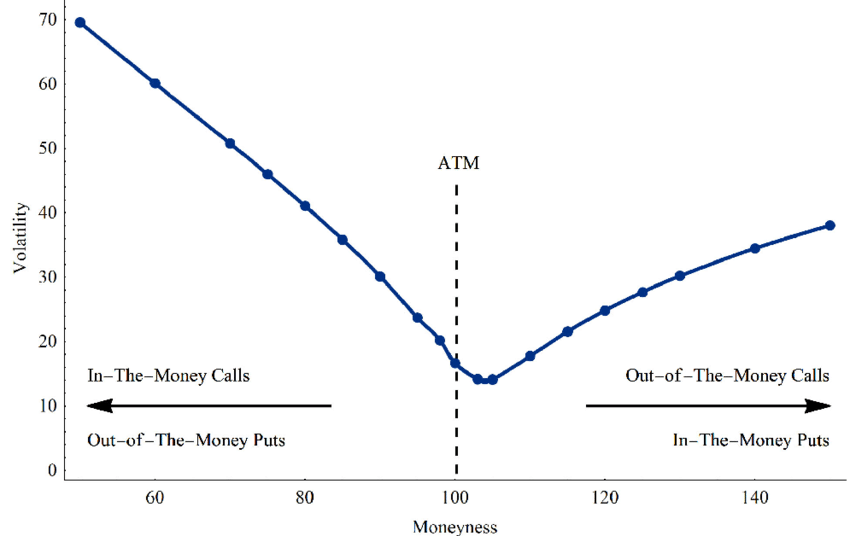
\includegraphics[scale=0.35]{images/Volatility-smile-SPX-Date-2018-11-17-Expiration-Date-2018-11-30-OTM-puts-are-in-less.png}
\caption{volatility smirk on the \code{SPX} dated \code{2018-11-30}}
\end{figure}

A 3-dimensional plot for each pair of $(T, K, \sigma_{imp})$ results in the so-called volatility surface. This is commonly used to give an understanding of market perspectives on the riskiness of particular options trades. The surface is also utilised  as input to risk management and hedging decisions. 

\newpage
\section{Observations of the Black-Scholes Model}
In the current state of quantitative finance, the Black-Scholes model serves as a benchmark rather than a state-of-the-art pricing solution. We summarise the strengths and weaknesses of the model. 

\subsection{Discrete Dividends}
We have so far only considered the case where an underlying stock pays a continuous dividend of $qS_t dt$. Over long time horizons (decades), it is often a reasonable approximation, though this is not convincing for short to medium term time periods. In practice, we must be able to handle the discrete nature of Dividends. \\
\\
For the remainder of the discussion we consider options contracts whose underlyings are Shares that pay a deterministic dividend of value $D$ at time $t_D$. Dividends are generally announced well in advance, typically one month, so this is a good model. 

\begin{figure}[h]
\centering
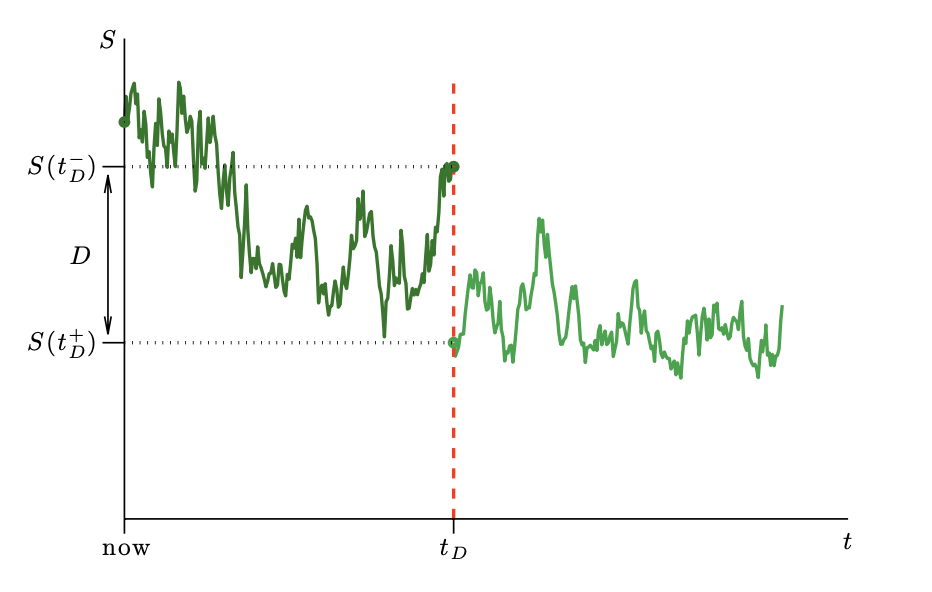
\includegraphics[scale=0.6]{images/DividendDate.png}
\caption{A jump in share price across a discrete dividend date}
\end{figure}
Note that under these assumptions we must have 
$S_{t_D^-} = S_{t_D^+} + D  \iff  S_{t_D^+} =  S_{t_D^-} - D $ otherwise there is an arbitrage opportunity.\footnote{}

\subsection{Geometric Brownian Motion}
One assumption that underpins the Black-Scholes model is that asset prices evolve according to the SDE 
$$\frac{dS_t}{S_t} = \mu dt + \sigma dB_t$$
Which has closed form solution 
$$S_t = S_0 \exp\left(\left(\mu-\frac{\sigma^2}{2}\right)^2t + \sigma B_t\right)$$
Which means for some $Z\sim N(0,1)$
\begin{align*}
    S_t &= S_0
\exp\left(\left(\mu-\frac{\sigma^2}{2}\right)^2t + \sigma \sqrt{t}Z\right)
\end{align*}
Recall that if $X\sim N(\mu,\sigma^2)$ then $Y=e^X$ follows a lognormal$(\mu, \sigma^2)$ distribution. Thus, when using geometric brownian motion to model asset prices, assets follow a lognormal$((\mu-\sigma^2/2)t, \sigma^2t)$ distribution.



\newpage
\section{Extension to America Options}
So far we have discussed the pricing formulae for European options, that offer a payoff of $\max(S_T-K,0)$ at time $T$ (for Call Options). American options, offer a more robust payoff, which allows the contract to be exercised at time $t\leq T$ for payoff $\max(S_t-K,0)$. \\
\\
In some markets, the volume traded on American options far exceeds that of Europeans, and naturally, an extension of the option pricing formula is desired for American payoff's. Suppose the option has payoff $P_A (S_t, t)$ which depends on time, $t$. Assuming we have no-arbitrage we must have \begin{itemize}
    \item The value of the option contract cannot be less then $P_A(S_t, t)$
    \item The American option cannot be worth less then an otherwise equivalent European option. 
    \item If the European option is always worth at least $P_A(S_t, t)$, then it is no worse to hold the option to expiry than to exercise it, so the price of the European and American options will agree.
\end{itemize}

\newpage
\section{Stochastic Volatility Models}

\end{document}